% Model Adaptation with Least-Squares SVM for Adaptive Hand Prosthetics
% Orabona, Castellini, Caputo, Fiorilla, Sandini
%
% A submission to ICRA 2009

\documentclass[conference,letterpaper,10pt]{ieeeconf}

\IEEEoverridecommandlockouts

\usepackage{times}
\usepackage{epsfig}
\usepackage{graphicx}
\usepackage{amsmath}
\usepackage[psamsfonts]{amssymb}
\usepackage{url}

% ------------ useful mathematical definitions

\def\RR{\mathbb{R}}
\def\NN{\mathbb{N}}
\def\xx{\mathbf{x}}
\def\ww{\mathbf{w}}
\def\aa{\boldsymbol{\alpha}}
\def\bb{\boldsymbol{\beta}}
\def\ee{\mathbf{e}}
\def\dd{\mathbf{d}}
\def\mdd{\tilde{\dd}}
\def\b{\mathcal{B}}
\def\d{\mathcal{D}}

\topmargin -35.0pt

\begin{document}

% ------------ frontmatter

\title{Model Adaptation with Least-Squares SVM\\for Adaptive Hand Prosthetics}

\author{Francesco~Orabona, Claudio~Castellini, Barbara~Caputo, Angelo~Emanuele~Fiorilla and Giulio~Sandini%
\thanks{F. Orabona \emph{(corresponding author)} and B. Caputo
  are with IDIAP,
  rue Marconi, 19, Case Postale 592, CH-1920 Martigny, Switzerland.
  e-mail: francesco.orabona@idiap.ch, barbara.caputo@idiap.ch}%
\thanks{C. Castellini
  is with the LIRA-Lab, University of Genova,
  viale F. Causa, 13, 16145 Genova, Italy.
  e-mail: claudio.castellini@unige.it}%
\thanks{A.E. Fiorilla and G. Sandini
  are with the DIST, University of Genova,
  viale F. Causa, 13, 16145 Genova, Italy.
  and the Italian Institute of Technology,
  via Morego, 30, 16163 Genova, Italy.
  e-mail: emanuele.fiorilla@iit.it, giulio.sandini@iit.it}%
}

\maketitle
\thispagestyle{empty}
\pagestyle{empty}

\begin{abstract}
  The dexterity of active hand prosthetics is limited not only due
to the limited availability of dexterous prosthetic hands, but
mainly due to limitations in interfaces. How is an amputee
supposed to command the prosthesis what to do (i.e., how to grasp
an object) and with what force (i.e., holding a hammer or grasping
an egg)? So far, in literature, the most interesting results have
been achieved by applying machine learning to forearm surface
electromyography (EMG) to \emph{classify} finger movements; but
this approach lacks, in general, the possibility of quantitatively
determining the force applied during the grasping act.

In this paper we address the issue by applying machine learning to the
problem of \emph{regression} from the EMG signal to the force a human
subject is applying to a force sensor. A detailed comparative analysis
among three different machine learning approaches (Neural Networks,
Support Vector Machines and Locally Weighted Projection Regression)
reveals that the type of grasp can be reconstructed with an average
accuracy of $90\%$, and the applied force can be predicted with an
average error of $10\%$N, corresponding to about $5$N over a range of
$50$N. None of the tested approaches clearly outperforms the others,
which seems to indicate that machine learning as a whole is a viable
approach.
%
%Notwithstanding the well-known bad conditioning of the surface EMG
%signal then, this looks highly encouraging in applying machine
%learning to enable amputees gain a fine control over advanced
%prosthetic hands, also since a surface EMG setup can be cheaply and
%easily realised and it is totally non-invasive.

\end{abstract}

% ------------ sections

\section{Introduction}
\label{sec:intro}
\section{Introduction/Motivation}
\label{sec:intro}

\dropcap{A}utomatic speech recognition (ASR) is the ability of a machine
to convert human speech, coded as an audio signal, into words.
Potential applications of ASR range from human-computer interfaces
to informatics for the disabled to data mining in large speech corpora.
Despite decades of research, state-of-the-art ASR
systems still need to be trained upon very large and heterogeneous data sets
to account for speech variability.
%, or upon a single speaker's speech in controlled conditions.
And nevertheless, human beings show an excellent ability
of understanding one another's speech, independently of the speaker, the
accent, the pitch and speed, noise, etc.

Recent neuroscientific
evidence indicates that the brain motor areas responsible for producing labial
and dental phonemes are also involved in their perception; D'Ausilio et al. \cite{dausilio}
show that in a discrimination task of /b/,/p/,/d/ and /t/, trans-cranial magnetic
stimulation of the lips and tongue \emph{motor areas} creates a bias in favor
of the \emph{perception} of labials, and similarly, stimulation of the tongue
favors dentals. This suggests that motor information may be paramount for
understanding speech in humans.

Inspired by these finding, in this paper we investigate whether the knowledge of speech production in humans 
integrated into an automatic phoneme classifier improves the identification in the acoustic dimension 
of the specific behaviors of the /b/,/p/,/d/ and /t/ plosive consonants.
 
In ASR, approaches that combine explicit speech production knowledge and audio features
have been proposed (see \cite{king} for a review) as alternatives 
to the classic approach  in which the complex acoustic effects of speech production variability 
(e.g., due to speaking rate) and coarticulation (the phenomenon by which the phonetic realization of a phoneme is affected by its phonemic context) are directly and implicitly modeled in the acoustic domain.

%Although conclusions on the actual utility of speech production knowledge are somehow contradictory

By limiting our investigation on the utility of motor information to the much simpler (than ASR) task of four consonants classification\footnote{Note that a recognition task requires both segmentation of speech into phones and their classification.} we are able to relax working assumptions and avoid technical difficulties that so far have hampered a satisfactory integration of motor information into ASR systems. 

Additionally, from previous work it is not feasible to properly identify which aspects of the recognition process benefit from motor information. For example, motor knowledge may improve the modeling (and so the identification) of coarticulation effects that are seen in the training data set, but not necessarily improve the recognition of phonemes in unseen contexts, i.e., it may not necessarily improve the generalization ability of the ASR system. On the other hand the experimental setup we have designed has the main goal of investigating whether motor information improves the generalization ability of a phoneme classifier.  

%Although the integration of speech production knowledge in an ASR system often brings some improvements, %it is commonly held that the potential of speech production knowledge is far from being exhaustively exploited.  

To this end, we have focused on the automatic version of
the problem tackled in D'Ausilio et al.'s work. For each consonant,
a corresponding typical phonetic motor invariant (MI) was
identified according to basic physiology of speech;
e.g., a fast, voiced opening (plosion) of the lips for /b/, and so on.
MIs were then used to semi-automatically segment the audio/motor data found in a
database of speech/motor trajectories recorded from $6$ subjects.

Subsequently, a simple regression method (namely, a feed-forward neural network) was employed
to build an Audio-Motor Map (AMM), which converts audio features of the isolated segment to
features of the related MI. On an abstract level, an AMM is a mathematical proxy of a mirror
structure \cite{umilta-01}, reconstructing the distal speaker's speech production act while
listening to the related piece of speech.

To test the approach, we have devised three experiments involving a 
classifier in the form of a Support Vector Machine \cite{BGV92}. We wanted to check whether
the use of MI-based features, either those recorded in the database (the ``real''
motor features) or the AMM-reconstructed ones (a more ecological scenario),
could improve the classifier's performance. Our results show that this is the case,
especially when the classifier is trained on incomplete data sets such as 
per-speaker (e.g., training on speakers $1,2,3$ and testing on $4$) and
per-coarticulation(e.g., training on /ba/, /be/, /bi/, /bo/ and testing on /bu/); or when noise is added,
in which case motor features significantly help classification, even when added to a
state-of-the-art set of audio features about $20$ times larger than that extracted
from the MIs.

\subsection{Related Work}

It is known since the Sixties \cite{liberman1} that the audio signal of speech
cannot be effectively segmented down to the level of the single phoneme,
especially as far as stop consonants such as bilabial plosives
are concerned; in particular, their representations in the audio domain are
radically different according to the phoneme which immediately follows.
It remains an open question then, how humans can
distinctly perceive a common phoneme, e.g.,/b/ in  /ba/ and /bi/, since they
apparently have access to the speaker's audio signal only.

The explanation put forward by the so-called motor theory of speech perception
(MTS, \cite{liberman2,galant}) is that, while perceiving sounds,
humans reconstruct \emph{phonetic gestures}, the physical acts of
producing the phonemes, as they were trained since birth to associate
articulatory gestures to the sounds they heard. 

Even ignoring the motor theory of speech perception the use of speech production knowledge is appealing in that the coupling of articulatory and audio streams allows for explicit models of the effects of speech production phenomena (e.g., coarticulation) on the acoustic domain. These effects cannot be precisely modeled (e.g., when the phoneme /a/ affects the phonetic realization of /b/ in /ba/?)  or modeled at all (e.g., what happens when I utter a /o/ with exaggeratedly open jaw?) when the phonemic stream is directly mapped onto the acoustic dimension as in the standard approach to ASR.  

Different solutions have been proposed to integrate speech production knowledge into an ASR system and different types of speech production information has been used, ranging from articulatory measurements (see \cite{zlokarnik,stephenson,wrench}, for example) to symbolic non-measured representations of articulatory gestures that "replicate" a (symbolic) phoneme into all its possible articulatory configurations\footnote{Articulatory configurations are configurations of the positions of the phonetic articulators} (see \cite{richardson, livescu}, for example).
 
   
%One possible reason why ASR is so difficult is then that
%machines have in general no access to the motor representation of the
%audio signal they are supposed to understand. We hypothesize that motor 
%information might help ASR, especially when tests on different speakers and different
%coarticulations are performed: for example, when training on subject $A$ and
%testing on subject $B$, or when training on pseudo-words such as /ba/, /bi/,
%/be/ and then testing for the presence of /b/ in /bo/, /bu/ or even /br/.

Although some studies have shown increased word recognition accuracy when including speech production knowledge in ASR, it is commonly held that the potential of speech production knowledge is far from being exhaustively exploited. Limits of current approaches include: the use of the phoneme as basic unit (as opposed to articulatory configuration, for example) which appears to be too "coarse", especially in the context of spontaneous spoken speech 
%where coarticulation effects are more frequent and marked
;and  the lack of a mechanism that accounts for the different importance of articulators in the realization of a given phoneme (e.g., in the generation of phoneme /b/ lips are critical, i.e., important, while tongue is non-critical).

The traditional approach in which the speech signal is segmented into phones, often referred to as "beads on a string" approach, poses problems to an accurate modeling of spontaneous speech where coarticulation phenomena such as phone deletion or assimilation (where a phone assimilates some articulatory gestures of the preceding/following phone), are frequent and not always predictable and call for finer-grained basic units (see \cite{ostendorf})). To partly make-up for such limitation we propose an alternative approach where, instead of segmenting the audio stream looking at audio features only and then observing the articulatory gestures within the identified phones, we give priority to the motor information in that speech is segmented by searching for phone-specific patterns of the (critical) articulatory gestures.

%Concerning the necessity of a phoneme dependent distinction between critical and non-critical articulators we do not 
%Traditionally (e.g., \cite{bourl,salvi}), the audio speech signal is segmented with a
%fixed-length Hamming window, usually 20ms. long. The resulting sequence
%is then analysed in the frequency or cepstral domain and the
%resulting coefficients are used as features for a classification system.
%One negative aspect of this approach is that it
%neglects the qualitative overall characteristics of the
%phoneme being uttered: depending on the speed of the speech, a consonant
%can have different lengths and, by using the above approach, global
%information about it is lost (see \cite{ostendorf}, where this approach is
%dubbed ``beads-on-a-string''). Nevertheless, as far as we know, there is
%so far no widely accepted alternative method for speech segmentation,
%if the audio signal is the only one available. One attempt, but not based
%upon articulatory data atl all, appears in \cite{bourlard}.


During recognition, articulatory gestures have to be recovered 
from audio information as audio is the only signal available.
Reconstruction of articulatory features has been attempted since a long
time, but in most cases it is not derived from articulatory \emph{data}
gathered from human subjects. One pioneeristic case is that of Papcun
et al. \cite{papcun} where the AMM is carried out by a Multilayer Perceptron.
Our procedure for building the AMM is deeply inspired by this work.
%By using a Multilayer Perceptron we implicitly assume that all articulators have the same importance and that the AMM is a %one-to-one mapping.   
%Papcun et al. \cite{papcun} observed that non-critical articulators have higher variance (in terms of position) than critical %articulators. 
The Multilayer Perceptron tries to carry out the best recovery of all articulatory gestures while more emphasis to the recovery of the gestures of the critical articulators should be given to the detriment of the non-critical articulators, which have higher variance (in terms of position, see \cite{papcun,rose}). Although we do not address this issue, the simple fact that we only consider two articulators alleviates a problem that would be otherwise far more relevant if all articulators were taken into account\footnote{The higher variance of the non-critical articulators is the main cause that makes AMM a one-to-many mapping: different articulatory configurations result in the same acoustic realization. Solutions to properly address this "ill-posed" nature of the AMM have been proposed by Richmond et al. \cite{richmond} and Toda et al. \cite{toda}. }.

%and subsequently Korin Richmond's work
%\cite{richmond2002,richmond2007} who have been able to reconstruct point-by-point
%the trajectories of articulators from the audio signal to a remarkably low
%error rate. The procedure for building the AMM is deeply inspired by their
%work.

Interestingly, the idea of using information about the mechanisms involved in the production of a human action to improve its classification/recognition (in a domain different from the production domain) has not only been applied in the context of speech recognition. For example Metta et al. \cite{metta-06} and Hinton \cite{hinton-2006} 
have shown that articulatory data can improve classification accuracy in automated hand action classification.

%TODO  
% Transferring the method to speech perception seems
% like a natural choice.


%\section{Problem Statement}
%\label{sec:prob}
%Our study mainly aims at answering the following question: can we
improve the training time a patient must undergo when learning to use
an adaptive prosthesis? In particular, since we have at our disposal a
data set gathered from $10$ subjects, can we somehow exploit the
analogies among the subject-wise data sets to build a model which will
give a headstart to the adaptation on a new, so far unseen patient?

Since we use machine learning, the question is equivalent to: can we
use model adaptation to obtain good results when these models are used
as a starting point for the adaptation on new data?

\textbf{BARBARA: ripensandoci questa sezione non mi convince. mi sa
che non ho granche' capito cosa volevi metterci...}


\section{Mathematical Framework}
\label{sec:math}
This section describes our mathematical framework. We first introduce
the basic notation (Section \ref{sec:back}), then we present our algorithm
for online model adaptation (Section \ref{sec:adapt}).

\subsection{Background}
\label{sec:back}

Assume $\xx_i \in \RR^m$ is an input vector and $y_i \in \RR$ is its
associated output.  Given a set $\{\xx_i,y_i\}_{i=1}^l$ of samples
drawn from an unknown probability distribution, we want to find a
function $f(\xx)$ such that it determines best
%determines 
the corresponding 
%associated 
$y$ for any future sample $\xx$.
%drawn from the same distribution.
This is a general framework that includes regression and
classification problems.  This problem can be solved in various
ways. Here we will use kernel methods and in particular Least-Square
Support Vector Machines (LS-SVM) \cite{Cristianini00}. In LS-SVM the
function $f(\xx)$ is built as a linear model $\ww \cdot \phi(\xx) +
b$, where $\phi(\cdot)$ is a non-linear function mapping input samples
to a high-dimensional (possibly infinite-dimensional) Hilbert space
called \emph{feature space}. Rather than being directly specified, the
feature space is usually induced by a \emph{kernel function}
$K(\xx,\xx')$ which evaluates the inner product of two samples in the
feature space itself,
%between the images of vectors in the feature space,
i.e. $K(\xx,\xx')=\phi(\xx) \cdot \phi(\xx')$. A common kernel
function is the Gaussian kernel
\begin{equation}
  K(\xx,\xx')=\exp(-\gamma ||x-x'||^2)
  \label{eq:rbf}
\end{equation}
\noindent that will be used in all our experiments.

The parameters of the linear model, $\ww$ and $b$, are found by
minimizing a regularized least-squares loss function
\cite{Cristianini00}. This approach is similar to the well-known
formulation of Support Vector Machines (SVMs), the difference being
that the loss function is the square loss.
%and it
While this does not induce a sparse solution,
% On the other hand 
it makes it possible to write the leave-one-out error in closed form
\cite{Rifkin07}. This is known to be approximately an unbiased
estimator of the classifier generalization error \cite{LuntzB69}. This
property is useful to find the best parameters for learning
(e.g. $\gamma$ in (\ref{eq:rbf})) and it will be used in our
adaptation method. Note that we use the same formulation to solve both
regression and classification problems.

\subsection{Model Adaptation}
\label{sec:adapt}

Let us assume we have $N$ pre-trained models stored in memory, trained
off-line on data acquired on $N$ different subjects. When the
prosthetic hand starts to be used by subject $N+1$, the system begins
to acquire new data. Given the differences among the subjects' arms
and as well in the placement of the electrodes, these new data will
belong to a new probability distribution, different from the $N$
previously modelled and stored. Still, as all subjects perform the
same grasp types, it is reasonable to expect that the new distribution
will be \emph{close} to at least one of those already modelled.
%We assume that the system has a number of previous models trained off-line on a
%number of different persons. The system then starts acquiring new data, coming
%from the person wearing the prosthetic hand. Given the differences in the
%electrodes placement and between the different subjects, the new data will
%belong to a distribution that is different from the ones of the other stored
%subject. Still we expect that the new distribution will be \emph{close} to at
%least one of the stored ones. 
Thus it should be possible to use one of the pre-trained model as a
\emph{starting point} for the training using the new data.
We expect that, by doing so,  learning should be faster
than using the new data alone. 
%Moreover the adaptation should not use the
%auxiliary data for training.
%FIXME FRA: frase ambigua, io la toglierei
To solve this problem we generalize the framework for adaptation proposed in
\cite{YangYH07} for SVM. 
%They propose 
The basic idea is to slightly change the regularization term of the
SVM, so that the solution will be close to the one of the pre-trained
model.  The optimization problem is \cite{YangYH07} %the following
\begin{align}
  \min_{\ww,b} \frac{1}{2} \|\ww- \ww'\|^2 + C \sum_{i=1}^N \xi^2 \nonumber \\
  \mbox{subject to} \;\;
  \xi_i \geq 0,\;\; y_i \ww \cdot \phi(\xx_i) + b \geq 1-\xi_i~,
  \label{eq:opt_prob_orig}
\end{align}
\noindent where $\ww'$ is one pre-trained model.
%In our opinion the above formulation has the disadvantage of giving a fixed
%weight to the previous model. 
This formulation gives a fixed weight to $\ww'$. This can be a
disadvantage in our scenario: for instance,
in the case none of the stored models is useful for the task at hand,
imposing the closeness could harm the performance of the new model.
To solve this problem, here we introduce a scaling factor for
the pre-trained model. In this way we can control the degree to which
the new model is close to the previous one.
We also change the loss into the standard square loss. This
gives us the possibility to calculate the leave-one-out error with a
closed formula, therefore
%and
%in this way 
to automatically tune this additional parameter. So we obtain the
following optimization problem
\begin{align} 
  \min_{\ww,b} \frac{1}{2} \|\ww- \beta \ww'\|^2 + \frac{C}{2} \sum_{i=1}^N \xi^2 \nonumber \\
  \mbox{subject to} \;\; y_i = \ww \cdot \phi(\xx_i) + b + \xi_i~.
  \label{eq:opt_prob}
\end{align}
It is easy to show that the optimal solution is %the form
\begin{equation}
  \ww = \beta \ww' + \sum_{i=1}^N \alpha_i \phi(\xx_i), \; \alpha_i \in \RR~,
\end{equation}
\noindent hence the final solution is given by the sum of the pre-trained model
scaled by the parameter $\beta$, and a new model given by the new data
points.  Note that when $\beta$ is $0$ we recover the original LS-SVM
formulation, that is without any adaptation to the previous data.  As
already mentioned, LS-SVM makes it possible to write the leave-one-out
error in a closed form. It turns out that it is possible to do the
same with the modified formulation (\ref{eq:opt_prob}). Hence it is
possible to set the parameter $\beta$ optimally, so to minimize the
leave-one-out error,
%. In particular
%for regression there is a closed formula for the optimal $\beta$. We leave the
%mathematical details for a longer version of this paper.
%Hence with a negligible additional computational cost we can choose the optimal
%value for the parameter $\beta$ and 
while at the same time we can choose the best pre-trained model for
adaptation.

As a last remark, we underline that the pre-trained model $\ww'$ can be
obtained by any training algorithm, as far as it can be expressed as a
weighted sum of kernel functions.  The framework is therefore very
general.


\section{Database}
\label{sec:mms}
%% To test the effectiveness of the approach we recruited $10$ healthy
%% subjects and recorded a dataset of more than $1200$'' of EMG and force
%% signals per subject.

\subsection{Subjects and setup}

%The experiment was carried out on 
We acquired data from ten healthy subjects, two women and eight men,
nine right-handed and one left-handed, of an average age of $30.9 \pm
8.45$ years. The subjects were generally na\"\i ve with respect to the
%experiment.
recording procedure. We placed on each subject's dominant forearm $7$
surface EMG electrodes. The number of electrodes and their positions
were chosen, visually and by palpation, according to the medical
literature \cite{Kendall}. This procedure allowed us
%in order 
to identify the most relevant flexor and extensor muscles of the
forearm, and to record their EMG activity from the spots that should
be least affected by signal cross-talk\footnote{But notice that some of the
aforementioned muscles are deep into the forearm, so that muscle
cross-talk cannot be completely avoided.}. The chosen locations were:

\begin{itemize}

  \item on the forearm ventral side: near the wrist, above the
     \emph{flexor pollicis longus}; centrally, above the \emph{flexor
     digitorum superficialis}; near the elbow, above the \emph{flexor
     digitorum profundus}; and near the wrist, above the \emph{flexor
     digitorum superficialis} again;

  \item on the forearm dorsal side: near the wrist, above the
     \emph{extensor pollicis brevis/abductor pollicis longus};
     centrally, above the \emph{extensor digitorum communis} and
     \emph{extensor digiti minimi}.

\end{itemize}

%\begin{figure*}[!t] \centering
%  \begin{tabular}{ccc}
%    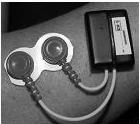
\includegraphics[height=0.16\textheight]{figs/Electrode} &
%    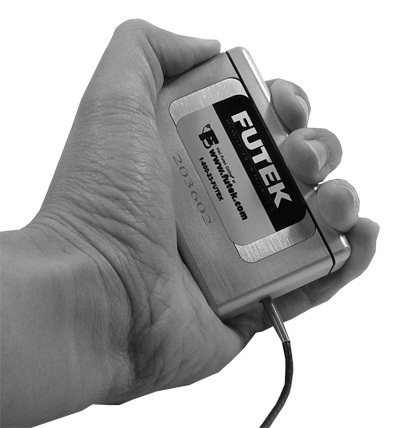
\includegraphics[height=0.16\textheight]{figs/Hand_Gripper} &
%    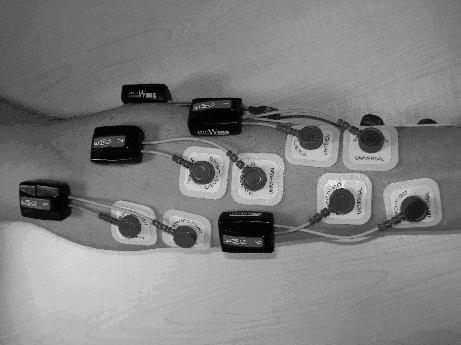
\includegraphics[height=0.16\textheight]{figs/El_Arrangement} \\
%    $(a)$ & $(b)$ & $(c)$ \\
%  \end{tabular}
%  \caption{The experimental setup (\textit{subject side}): $(a)$ an EMG
%    wireless electrode; $(b)$ the FUTEK force sensor; $(c)$ the typical
%    placement of the EMG electrodes on a subject's forearm (ventral side).}
%  \label{fig:SubjSetup}
%\end{figure*}

We employed the electrodes Aurion ZeroWire wireless EMG electrodes
%electrodes (see 
\cite{zerowire}. 
%The use of wireless electrodes helped the subjects
%freely move, to mimic their Daily-Life Activities (DLAs) during the
%acquisition.
%, not beeing wrapped in a thick net of electric cables. 
Moreover the subjects were given a FUTEK LMD500 Hand Gripper force
sensor \cite{LMD500} in order to measure the force applied by her/his
hand during the recording.

%Figure \ref{fig:SubjSetup} shows $(a)$ a single electrode, glued to the subject's forearm skin; $(b)$ the force sensor as gripped during a power grasp; and $(c)$ the typical placement of the electrodes (ventral side of the forearm).

We used a standard National Instruments data acquisition board
(NI-USB6211) connected to the receiver of the EMG wireless device and
to the force sensor, in order to record the sensors' signals and the
exerted force. We set the sampling rate of the board at $2$kHz, since
it is known that the raw EMG relevant bandwidth lies between $15$ and
$500$Hz. See Figure \ref{fig:spectra} for an example.
% To avoid synchronisation problems, we chose to record also
% the signal coming from the Hand Gripper at same sampling rate.

%The board was connected via a USB port to a custom National Instruments' LabView VI application (running on an entry-level laptop) to acquire all the signals.

\subsection{Data acquisition and pre-processing}
\label{sec:preproc}

%First of all we decided to record a rest condition to define the baseline of the EMG activity, than we started the experiment. 
We first considered a rest condition, so to define the baseline of the
EMG activity. We then proceded with the data recording:  
%It consisted
%of two phases, one right after the other:
%
%\begin{itemize}
%
%  \item Phase $1$: 
the subject kept her/his arm still and relaxed on a
    table, and was asked to grasp the force sensor using, in turn,
    three different grips (Figure~\ref{fig:Grasps}).
%
%  \item Phase $2$: the subject was asked to grasp the force sensor (as
%    she/he did in the previous phase) while freely moving, walking
%    around, lifting and pronating/supinating the arm and forearm,
%    sitting down and standing up from a chair. This should emulate the
%    main movements that one is expected to do during DLAs.
%
%\end{itemize}
%
%From now on, the two phases will be referred to as \emph{Still-Arm
%phase (SA)} and \emph{Free-Arm phase (FA)} respectively.

\begin{figure*}[!ht] \centering
  \begin{tabular}{ccc}
   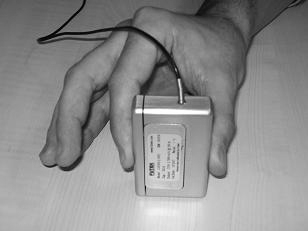
\includegraphics[height=0.16\textheight]{figs/grip1} &
    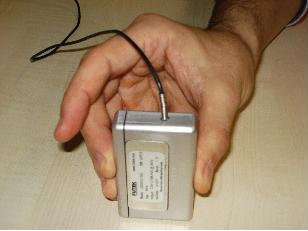
\includegraphics[height=0.16\textheight]{figs/grip2} &
    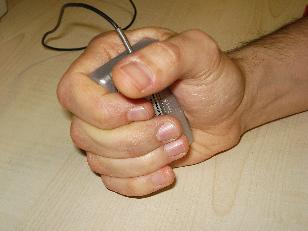
\includegraphics[height=0.16\textheight]{figs/grip3} \\
    $(a)$ & $(b)$ & $(c)$ \\
  \end{tabular}
  \caption{The three different grips employed in the experiment: $(a)$
   index precision grip; $(b)$ other fingers precision grip; $(c)$
   power grasp.}
  \label{fig:Grasps}
\end{figure*}

\begin{figure*}[!ht] \centering
  \begin{tabular}{cc}
    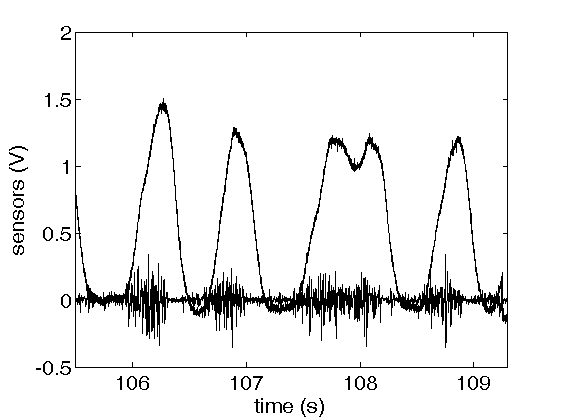
\includegraphics[width=0.45\textwidth]{figs/force_raw} &
    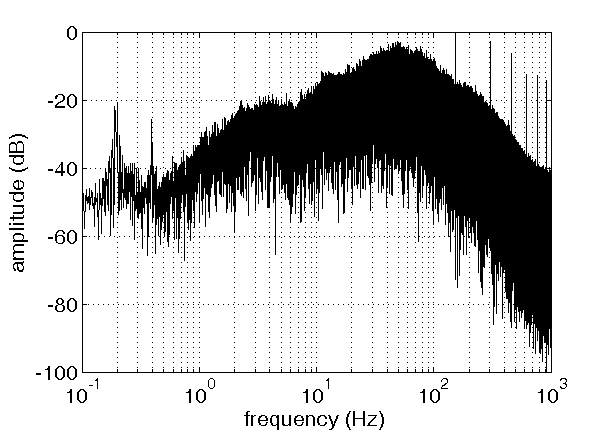
\includegraphics[width=0.45\textwidth]{figs/spectrum_raw} \\
    $(a)$ & $(b)$ \\
  \end{tabular}
  \caption{$(a)$ typical raw EMG and force signals; $(b)$ frequency diagram of
    the EMG signal.}
  \label{fig:spectra}
\end{figure*}

%During each phase,
The subject freely repeated each grasping action
for $100$'', resting for $30$'' in between grasps. In order to gather
more data and diminish the effect of local errors, the whole procedure
was repeated twice. As a whole, each subject's recording resulted in
about $2.4\times 10^6$ samples. 
%equally distributed in each phase.

Unlike commercial EMG electrodes, such as, e.g., Otto Bock's MyoBock
electrodes \cite{ottobock} that return the on-board computed Root-Mean
Square (RMS) of the EMG signal, the electrodes employed here return
the ``raw'' EMG signal.
% within 10Hz and 1kHz.
%without any low-pass filtering or Root-Mean Square (RMS) processing.
Nevertheless, it is well-known \cite{deluca,zecca} that the force
exerted by a muscle is strongly related to the RMS of the EMG signal,
rather than to the raw signal. For this reason, in order to have a
signal that is as similar as possible to a \emph{control signal}, we
decided to evaluate the RMS, electrode by electrode.

For a given mono-variate discrete time-varying signal, the RMS is
defined as the mean of the squares of the signal values, evaluated
over a certain time-window $T_{RMS}$. Roughly speaking, the RMS acts
like an envelope extraction plus a low-pass filter, whose cutoff
frequency grows smaller as the time-window grows larger (i.e., as
$T_{RMS}$ becomes higher). For this reason, high values of $T_{RMS}$
imply an ostensible delay in the resulting signal that is due to
\emph{responsiveness} of the synthesized output signal.  It becomes
slower and slower as the $T_{RMS}$ value increases, since more
``samples'' are averaged to obtain a significant value. The choice of
$T_{RMS}$ is therefore crucial to produce a signal which is maximally
related to the force signal, unaffected by high-frequency noise, and
with an acceptable lag. However, it must be noted here that the EMG
signal, being directly related to the muscle \emph{activation
potentials}, happens to \emph{anticipate} the muscle
movements\footnote{The electromechanical delay (EMD) of a muscle is
defined as the interval between the onset of the electrical activity
of the muscle (EMG) indicating its activation by the neural system and
the onset of the resulting change in the mechanical variable
observed. The delays reported range from 25 to 100ms for different
muscles and tasks \cite{Wolf1994}.}. Therefore, in practical
applications, it can be considered as acceptable a wider lag than what
one would expect.
%a wider lag is acceptable than one would expect. 
This is useful since it allows us to increase $T_{RMS}$, if necessary.

%\begin{figure*}[!ht] \centering
%  \begin{tabular}{ccc}
%    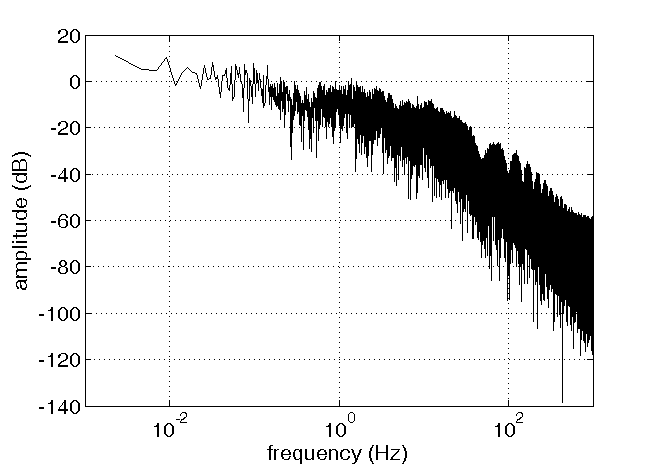
\includegraphics[width=0.3\textwidth]{figs/spectrum_RMS0040} &
%    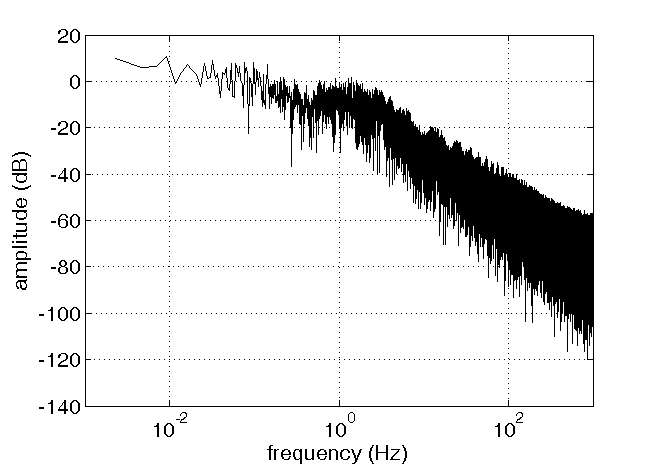
\includegraphics[width=0.3\textwidth]{figs/spectrum_RMS0200} &
%    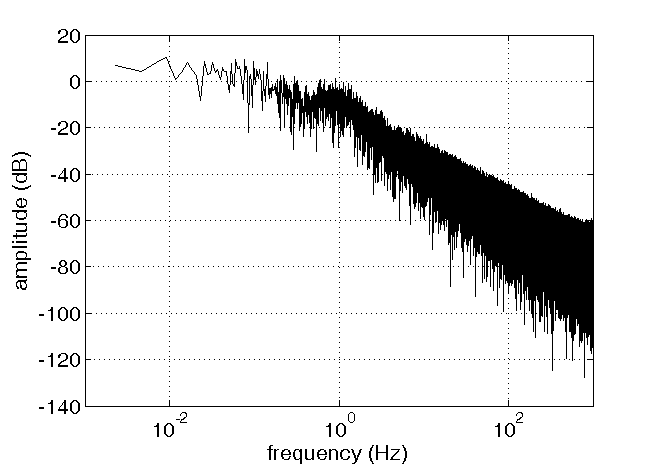
\includegraphics[width=0.3\textwidth]{figs/spectrum_RMS1000} \\
%    $(a)$ & $(b)$ & $(c)$ \\
%  \end{tabular}
%  \caption{(left to right) effects of the RMS on the bandwidth of the EMG
%    signals, for $T_{RMS} = 20, 100, 500ms$.}
%  \label{fig:RMSs}
%\end{figure*}

%Unfortunately 
We are not aware of any systematic way of setting a good value of
$T_{RMS}$ in such a framework. Therefore we found $T_{RMS}$
heuristically, according to some initial experiments.
% As an example, though, consider Figures \ref{fig:spectra} and \ref{fig:RMSs}.

Figure \ref{fig:spectra} (panel $(a)$) shows a few seconds of typical
force/EMG behavior: it is apparent that the EMG signal starts oscillating when the force signal
starts increasing. It is also quite clear that the
amplitude of the envelope of the EMG is related to the force, as
indicated in the literature. Panel $(b)$ shows the frequency analysis
of the same EMG signal: as one can see, the meaningful bandwidth lies
in the interval known from the literature.

%On the other hand, Figure \ref{fig:RMSs} shows the effect of the RMS on the frequency components of the EMG, for three different values of $T_{RMS}$.
%It is clear that the meaningful bandwidth now contains all low-frequency components, possibly down to the constant, and is upper-bounded by about $25$Hz (panel $(a)$, for $T_{RMS}=20ms$) to $10$Hz (panel $(c)$, for $T_{RMS}=0.5s$). As expected, larger values of $T_{RMS}$ correspond to a better filtering but also to a larger delay.

This enables us to safely sub-sample the EMG signal after having
applied the RMS. Assuming that $T_{RMS}$ is not too small, we
subsampled both the EMG and force signal at $25$Hz, taking one sample
every $80$ of the original sequence.  This considerably reduced the
amount of data to be processed, namely to about $30.000$ samples for
each subject.

As a last data pre-processing step, we removed from the sample set
those samples for which the applied force was lower than a specific
threshold, in order to get a clearer representation of the activation
potentials. This threshold was chosen in order to remove a minimal
fraction of the samples. Of course, we fully retained the samples
corresponding to the baseline rest condition.  This is why we chose to
record this condition before the data acquisition.
%rest of the experiment.


\section{Experimental Results}
\label{sec:exp}
We conducted two different experiments, one to predict the force measured
by the force sensor and another one to classify the grasp type.
The EMG data were the preprocessed as described in Section \ref{sec:preproc}.

As already mentioned in Section \ref{sec:adapt}, our working assumption is to have
 $N$ pre-trained models stored in memory.
Then new data comes from subject $N+1$ and the system starts
training, to build the $N+1$ model.
The performace is evaluated using unseen data from the subject
$N+1$.
To simulate this scenario and to have reliable estimation of the
performance, we used a leave-one-out approach: 
of the 10 subjects for which we have the data recordings, we train off-line
9 models. These will correspond to the $N$ stored models in memory. The data from the 10th 
remaining subject will be used for the adaptive learning of the $N+1$ model.
The training sequences are random subsets from the entire dataset, that is taken without
considering the order in which they were acquired.
This procedure is repeated 10 times, using in turns all the recorded subjects
for the adaptive learning of the model.

To assess the performance of the proposed adaptation method we compared it
to two baseline methods. The first one, that we call \emph{Prior}, consists in
using only the pre-trained models without updating them with the new training data.
Then we consider only the best performance of the 9 pre-trained models, to consider
the best-case scenario.
The second one, \emph{NoAdapt}, consists in using LS-SVM using only the new data
for training, as it would be in the standard scenario without adaption.
For classification we used the classification rate as a measure of
performance; for regression, the performance index is the correlation coefficient
evaluated between the predicted force signal and the real one. The
choice of the correlation coefficient, as opposed to the more standard
Mean-Square Error, is suggested by a practical consideration: when
driving a prosthesis, or even a non-prosthetic mechanical hand, we are
not interested in the absolute force values desired by the
user/subject, since mechanical hands usually cannot apply as much
force as human hands do, for obvious safety reasons\footnote{or, e.g.,
in teleoperation scenarios, they could be able to apply \emph{much
more} force than a human hand can.}. We are rather concerned about
getting a signal which is \emph{strongly correlated} with the
user/subject's will.
To build the  pre-trained models we used the standard SVM algorithm. All the parameters to be set during %of the
training ($C$ and $\gamma$ of the gaussian kernel) were chosen by cross-validation.

Figure \ref{fig:diff_cla} shows the average difference between 
the classification performance of \emph{NoAdapt} and our method. We see that using our adaptation
method there is always an improvement in performance, but when training is done on too little samples %are too
%few 
the standard deviations are big, i.e. depending on the subject there can be both a great gain or loss in performance. 
This is due to the high variance of the
leave-one-out error with few training samples. Still, the average gain is
almost $5\%$ when there are only 30 training samples and it seems to stabilize
around $1\%$ as the training samples increase.
Figure \ref{fig:cla_abs}.a shows the best performance obtained by our method
on a particular subject, while  Figure \ref{fig:cla_abs}.b shows the worst
performance achieved, of course on another subject. We see that in the best case the gain is quite significant,
while in the worst case we basically obtain  the performance of \emph{NoAdapt}. This last case is an example
where none of the models stored in memory matched the new distribution of the data, so the parameter
$\beta$ is automatically set to a very small value and in practice there is no transfer of prior knowledge. It is reasonable to think
that the performance of the method would increase with the number of stored
models, as it would increase the probability to find a good pre-trained model.
Note that in all the cases the performance of \emph{Prior} models, where well
below the performance of \emph{Adapt} and \emph{NoAdapt}: in Figure \ref{fig:cla_abs} is shown
only the performance of the best one among all the 9 stored models.
Similar observations can be done for the regression task in Figure \ref{fig:diff_reg}
and Figure \ref{fig:reg_abs}. In particular we gain in average 0.05 points on the score
of the correlation coefficient on the first 30 samples. Then the gain seems to decrease,
maybe approaching 0 when enough new training samples are acquired. However note that
the standard deviation bars are all above the zero, meaning that in worst case most of the time
we do not lose anything compared to the NoAdapt model (cf. Figure \ref{fig:reg_abs}.b).

\begin{figure}[t]
  \centering
  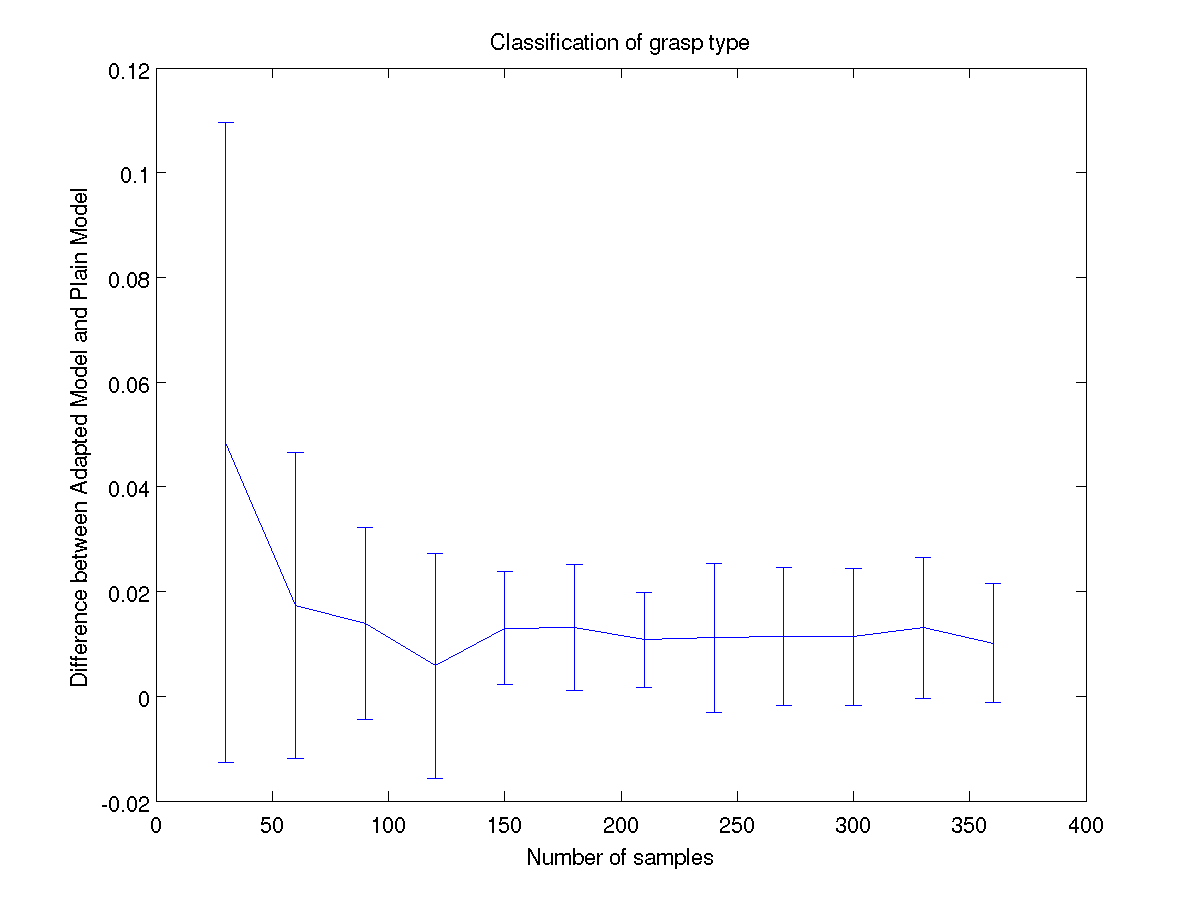
\includegraphics[width=0.95\linewidth]{figs/exp1}
  \caption{Classification results: Difference in performance between \emph{NoAdapt} and our method  on the
 classification of the grasp types.}
  \label{fig:diff_cla}
\end{figure}

\begin{figure*}[ht] \centering
  \begin{tabular}{cc}
    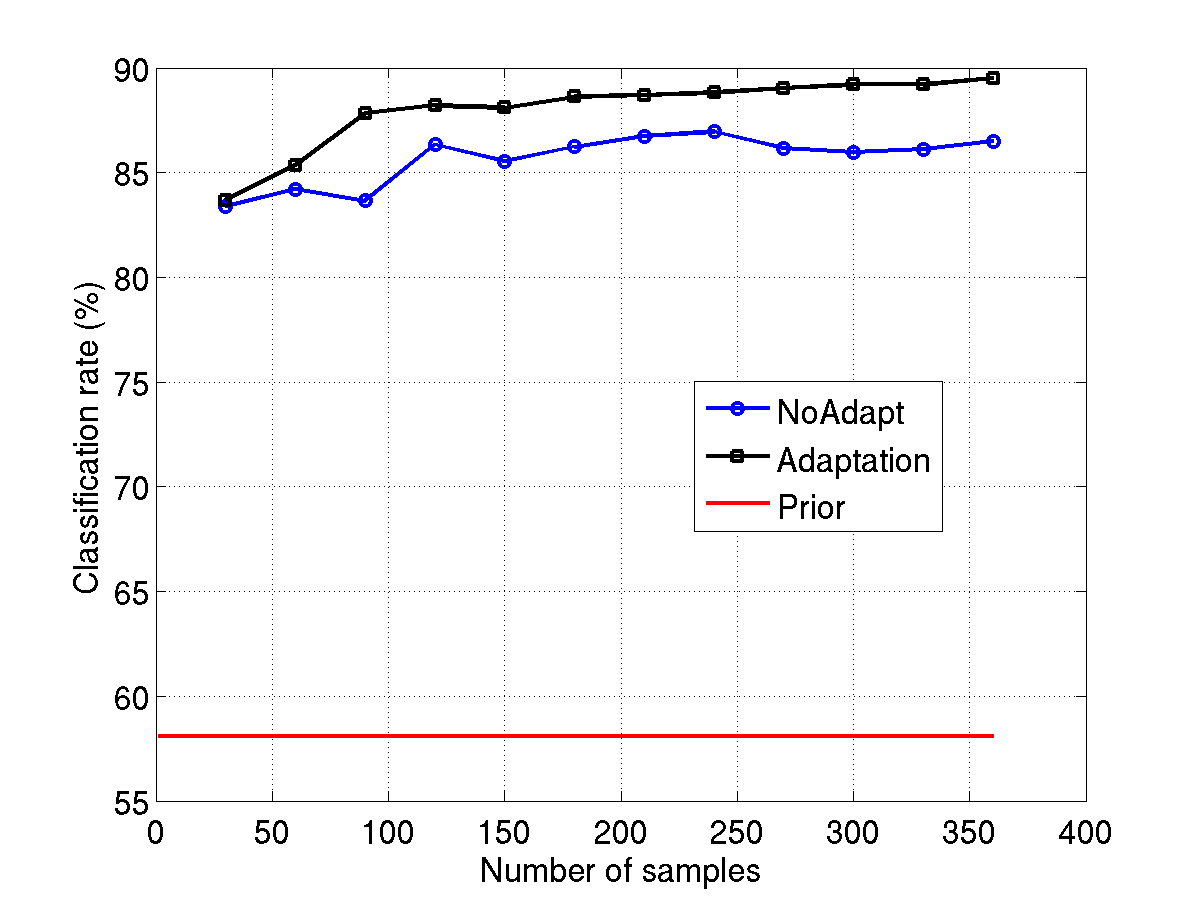
\includegraphics[width=0.45\textwidth]{figs/exp1_abs_best} &
    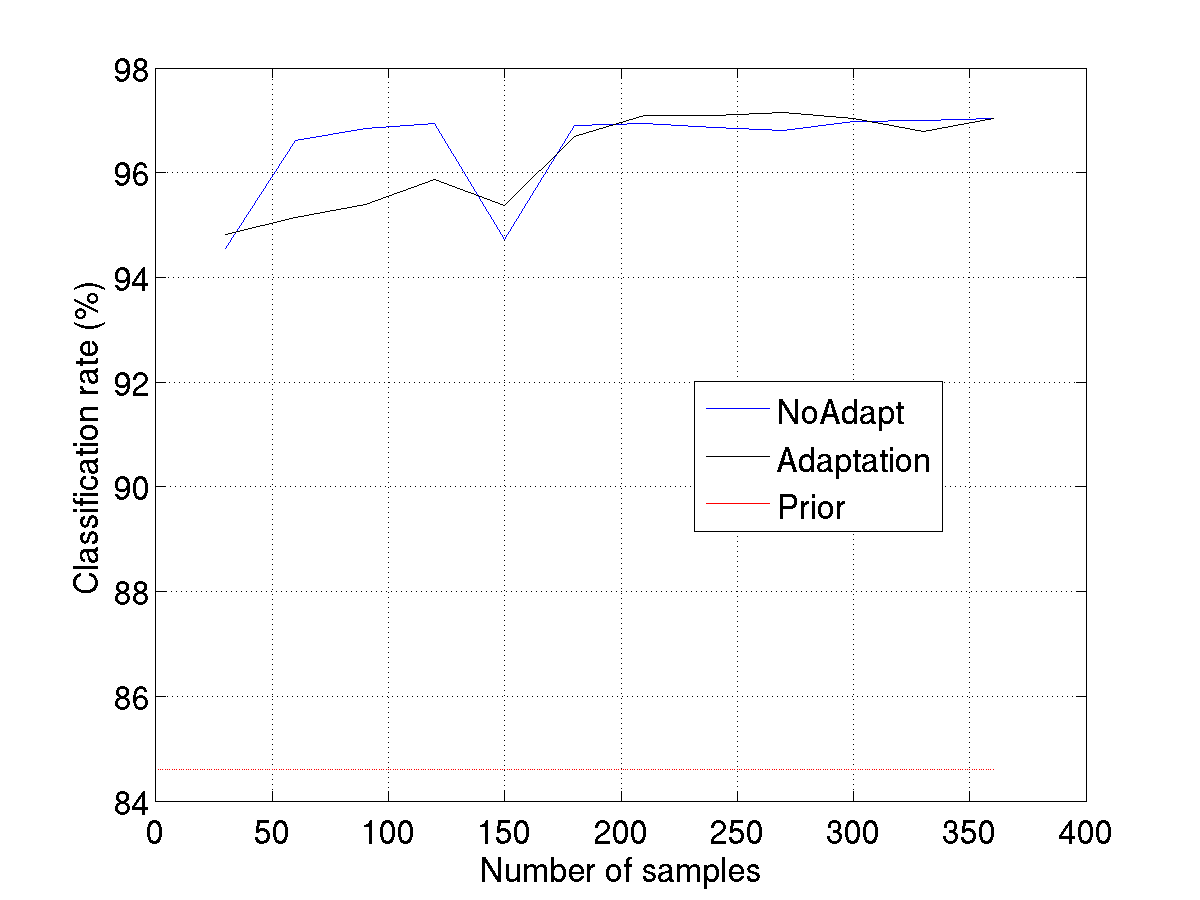
\includegraphics[width=0.45\textwidth]{figs/exp1_abs_worst} \\
    $(a)$ & $(b)$ \\
  \end{tabular}
  \caption{Classification results: $(a)$ Best classification rate gain of the adapted model compared to
 \emph{NoAdapt} and \emph{Prior} on a particular subject; $(b)$ worst performance on another subject.}
  \label{fig:cla_abs}
\end{figure*}

\begin{figure}[ht]
  \centering
  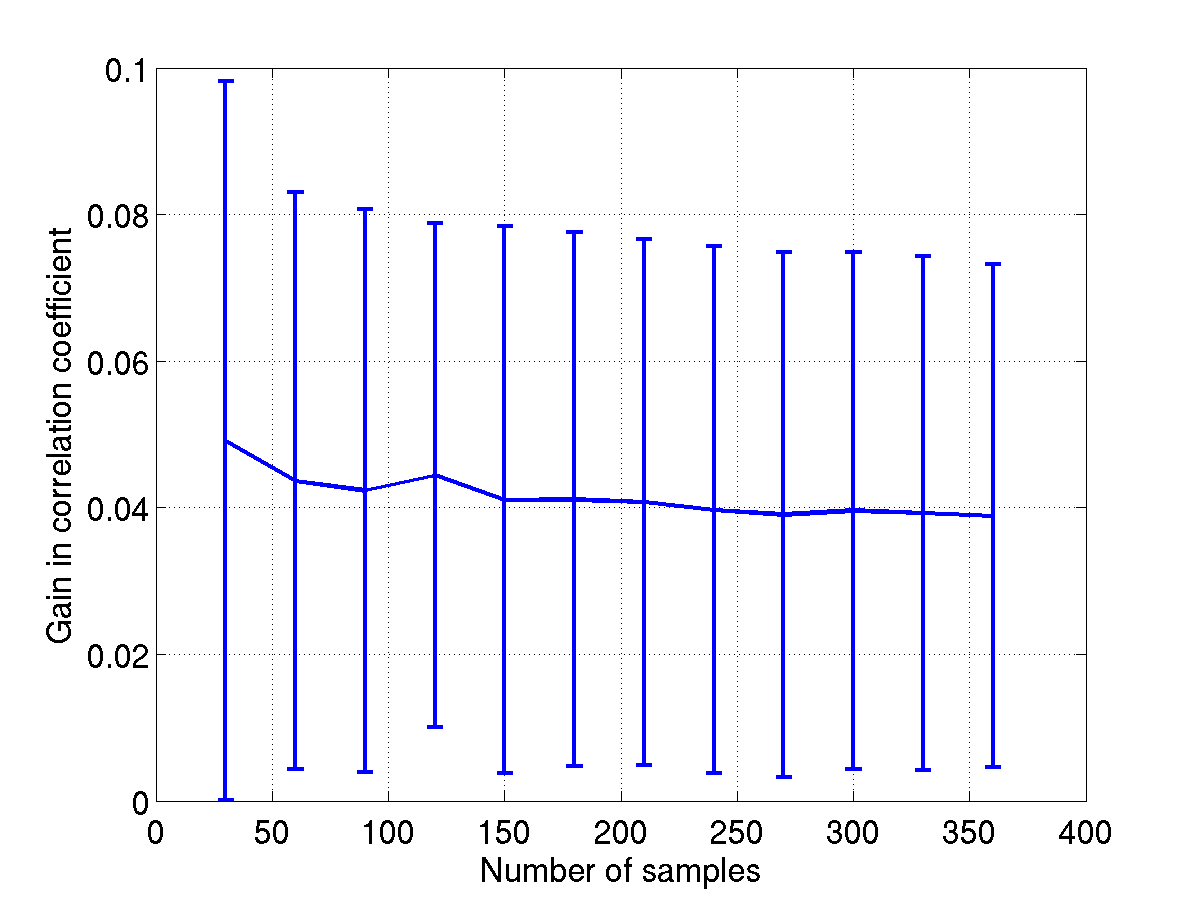
\includegraphics[width=0.95\linewidth]{figs/exp2}
  \caption{Regression experiments: Difference in performance between \emph{NoAdapt} and our method  on the
 regression of the force.}
  \label{fig:diff_reg}
\end{figure}

\begin{figure*}[ht] \centering
  \begin{tabular}{cc}
    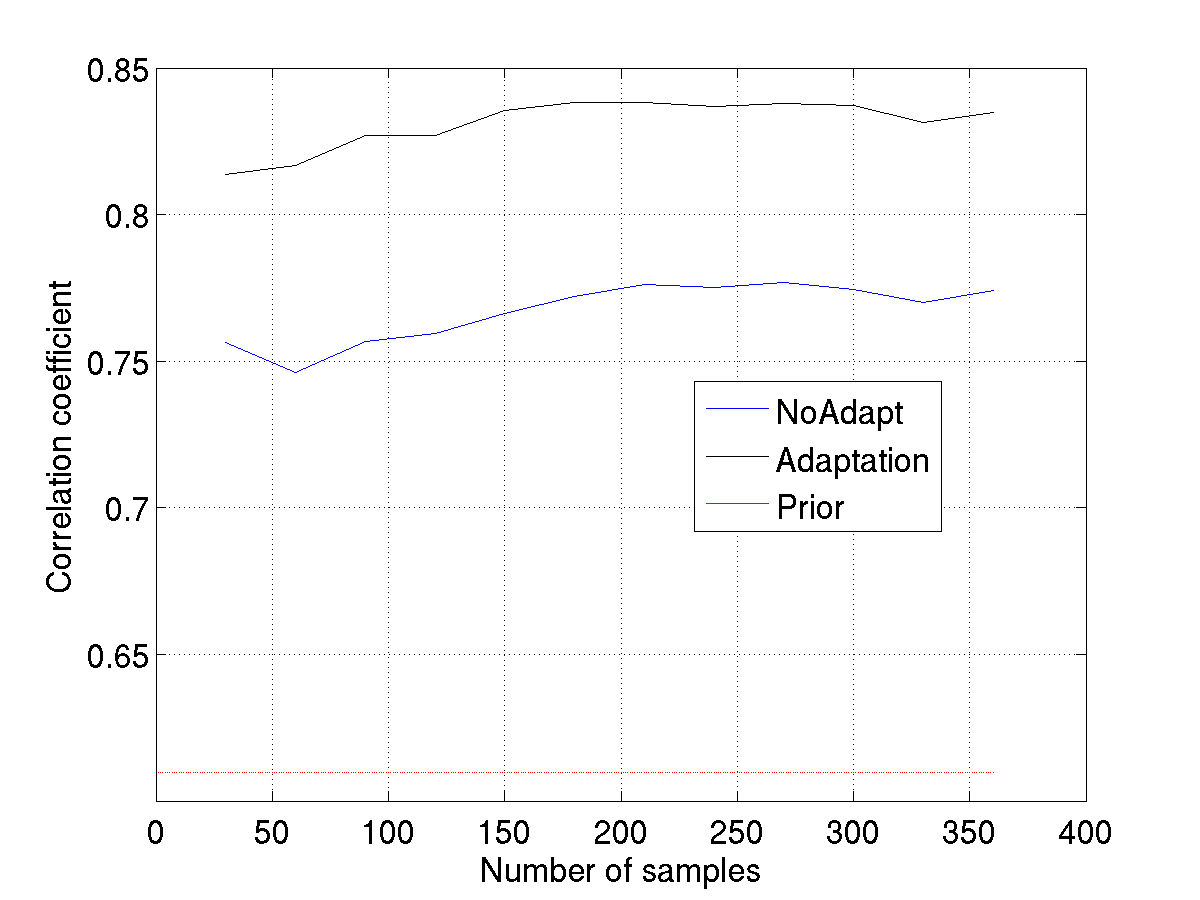
\includegraphics[width=0.45\textwidth]{figs/exp2_abs_best} &
    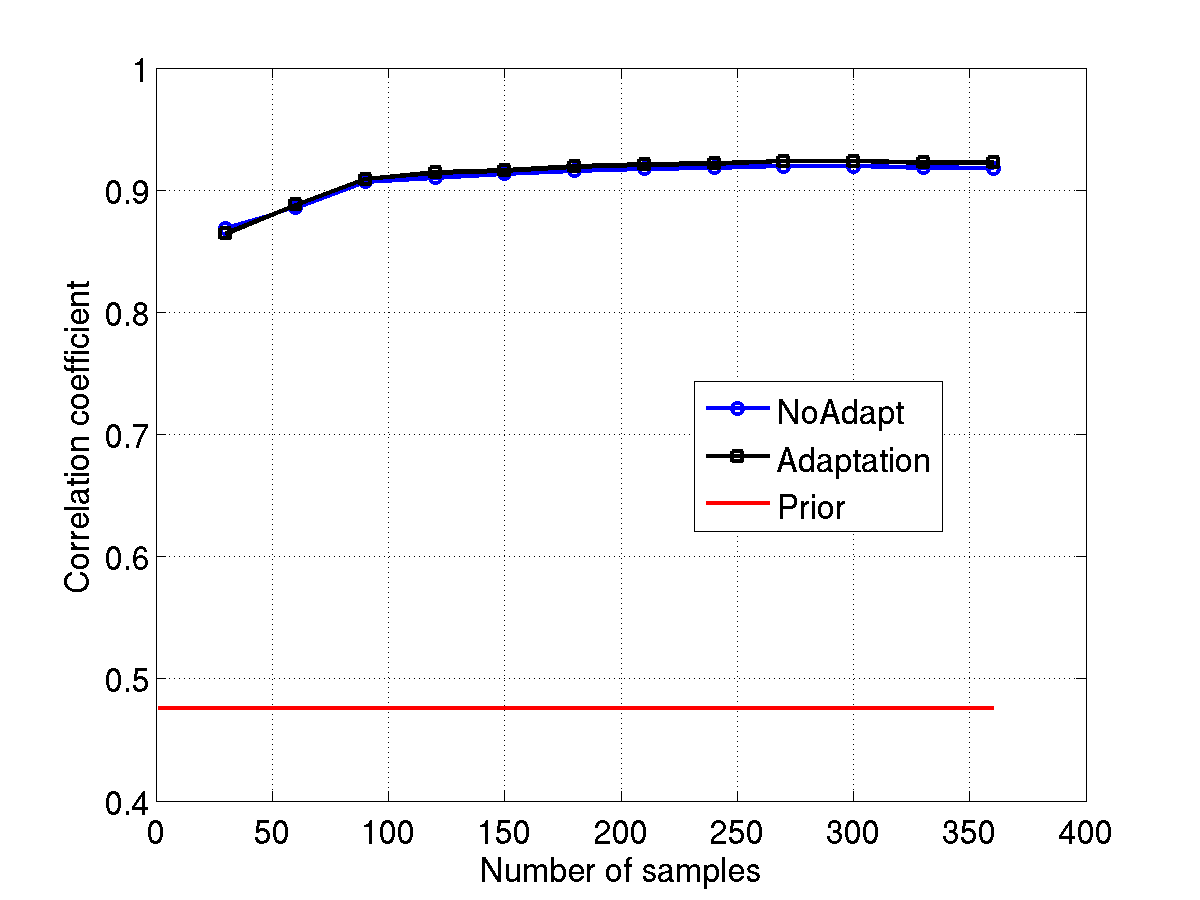
\includegraphics[width=0.45\textwidth]{figs/exp2_abs_worst} \\
    $(a)$ & $(b)$ \\
  \end{tabular}
  \caption{Regression experiments: $(a)$ Best correlation coefficient gain of the adapted model compared to \emph{NoAdapt}
 and \emph{Prior} on a particular subject; $(b)$ worst performance on another subject.}
  \label{fig:reg_abs}
\end{figure*}


\section{Conclusions}
\label{sec:concl}
The model adaptation method presented in this paper stems from a
problem in adaptive hand prosthetics, namely: is it possible to help a
patient to learn to use a dexterous hand prosthesis 
%in a quicker and
%better way, 
by exploiting the common features found in models trained upon other
patients?
The answer, at least as far as healthy subjects are concerned, is yes:
we have hereby presented a novel method for model adaptation in
machine learning, using Least-Squares SVMs; the idea is to build a SVM
solution which is \emph{close} to one of a set of pre-stored
models. The choice of which model to use among the pre-trained ones,
as well as the parameter $\beta$, determining the degree of closeness
to start the training from, are completely automatic, as we use an
estimation of the generalization error.

We tested our method on a database built with EMG and force data from
$10$ healthy subjects, trying to improve the training times and
asymptotic performance of one subject by pre-training on other
subjects. The outcome of the experiment is positive: our method gains
consistently both in the classification and regression tasks in the
best and average cases, and it resorts to the non-adaptive performance
in the worst.

Therefore, it is apparent that a large amount of knowledge stored in
LS-SVM models is common to all subjects, which is obviously due to the
analogies among the tasks performed by the subjects, as well as to the
anatomical similarities among the arms and the careful positioning of
the electrodes on the subjects' forearms. A further interesting point
is that, almost uniformly, models obtained by adaptation from a
pre-trained model obtain a \emph{better} performance than those
trained from scratch. This result is somehow surprising, although very
encouraging, and subject of future research.

Notice that we present no results on a real prosthetic/robotic hand so far --- this is subject of immediate-future research. We successfully applied a similar system to the DLR-II mechanical hand (see \cite{2008.ICRA,2008.BioCyb}), and since the accuracy of the system presented here is analogous to that of the one therein, there is no reason why the results presented here should not apply as well in the practical case. One interesting possibility is that of using this system to speed up the adaptation of an already existing dexterous hand prostheses, such as, e.g., Touch Bionics's i-LIMB \cite{ilimb} prosthetic hand, as already mentioned in the introduction.

Lastly, let us consider the fact that, most likely, the overall
performance of the method will increase when more subjects are
available, since this would mean a larger probability of finding a
matching pre-trained model. In a clinical setting, this means that
after an experimental phase, adaptive prostheses employing this method
could actually be built. It remains, of course, to discover whether
this idea can be transferred to amputees: amputations are, obviously,
non-controlled, traumatic events (except in some cases), and therefore
stumps exhibit much more variability than healthy forearms. This is
the subject of ongoing as well as future research.


% ------------ acks, biblio, biographies

\section*{Acknowledgments}

This work is partially supported by the project NEURObotics,
FP6-IST-001917 (C. C., ???) and the project DIRAC FP6-IST-027787 (F. O., B. C.). We thank Thierry Pozzo and Marco Jacono of IIT,
Genova, Italy, for their support during the experiment.

{\small
\bibliographystyle{IEEEtran}
\bibliography{paper,claudio}
}

\end{document}
